\documentclass[a4paper,10pt]{article}

\usepackage{booktabs}
%\usepackage{multirow}
\usepackage{tabularx}
\usepackage{geometry}
\usepackage{graphicx}
\geometry{
    a4paper,
    left=1cm,
    right=1cm,
    top=1cm,
    bottom=2cm}
\usepackage{xepersian}
\settextfont{Vazirmatn-Regular.ttf}


\title{گزارش روش طراحی معماری سیستم هوش مصنوعی بر اساس ساختار IMO Model-Output) (Input-AI برای پذیرش موفقیت‌آمیز هوش مصنوعی در سازمان‌ها}
\author{محمد خورشیدی روزبهانی\\40215741002013 \and شارا شاهوردیان\\40215741002032 \and ملیکا محمدی گل\\40215741002066}
\date{}

\linespread{1.5}

\begin{document}

    \maketitle

    \vspace{0.5cm}

    \begin{abstract}
        
        با پیشرفت فناوری هوش مصنوعی، بهبود موفقیت فناوری هوش مصنوعی در سازمان‌ها اولویت اصلی جامعه مدرن شده است. با این حال، بسیاری از سازمان‌ها هنوز به بیان فناوری های هوش مصنوعی لازم و کارشناسان هوش مصنوعی دچار مشکلات در فهم مسائلی که این سازمان‌ها با آنها روبرو هستند، دچار مشکل هستند. این شکاف دانشی باعث می‌شود که برای سازمان‌ها امکان شناسایی نیازهای فنی، مانند داده‌ها و الگوریتم‌های لازم برای اتخاذ فناوری هوش مصنوعی، مشکل باشد. برای پاسخ به این مشکل، ما یک روش طراحی معماری سیستم هوش مصنوعی جدید بر اساس ساختار IMO (ورودی-مدل هوش مصنوعی-خروجی) پیشنهاد می‌دهیم. ساختار IMO امکان شناسایی موثر نیازهای فنی لازم برای توسعه مدل‌های واقعی هوش مصنوعی را فراهم می‌کند. در حالی که تحقیقات قبلی اهمیت و چالش‌های نیازهای فنی، مانند داده‌ها و الگوریتم‌های هوش مصنوعی، برای اتخاذ فناوری هوش مصنوعی را شناسایی کرده‌اند، تحقیقات کمی در زمینه روش‌شناسی برای تجسم آنها صورت نگرفته است. روش‌شناسی ما از سه مرحله تشکیل شده است: تعریف مسئله، راه‌حل AI سیستم، و راه‌حل فنی هوش مصنوعی برای طراحی فناوری و نیازهایی که سازمان‌ها به صورت سیستمی نیاز دارند استفاده می‌کند. اثربخشی روش ما از طریق یک مطالعه موردی، تحلیل مقایسه‌ای منطقی با دیگر مطالعات، و بررسی توسط کارشناسان، که نشان می‌دهد روش ما می‌تواند به موفقیت اتخاذ فناوری هوش مصنوعی در سازمان‌ها کمک کند، اثبات شده است.

    \end{abstract}

    \section{مقدمه}

        همچنان که فناوری هوش مصنوعی پیشرفت می‌کند، اتخاذ موفق فناوری هوش مصنوعی برای بسیاری از سازمان‌ها اولویت اصلی شده است. با اتخاذ فناوری هوش مصنوعی، سازمان‌ها می‌توانند ارزش کسب و کار جدیدی ایجاد و به بهره‌وری و کارآمدی در تصمیم‌گیری‌ها افزوده شود [51،52]. به عنوان یک نتیجه، تلاش‌ها برای ترویج تحول و نوآوری سازمانی به سوی اتخاذ فناوری‌های هوش مصنوعی، نه تنها در شرکت‌های دیجیتالی مانند مایکروسافت یا نت‌فلیکس، بلکه در سازمان‌های سنتی مانند صنایع دفاع و راه‌آهن نیز تقویت می‌شود [53]. به عنوان مثال، در سال ۲۰۱۸، وزارت دفاع ایالات متحده مرکز هوش مصنوعی مشترک (JAIC) را تأسیس کرد، یک دپارتمان مخصوص برای اتخاذ فناوری هوش مصنوعی در تمام زمینه‌های دفاعی [33]. با این حال، طبق تحقیقات معتبری مانند گارتنر و مک‌کینزی، بسیاری از سازمان‌ها با مشکلاتی در اتخاذ فناوری هوش مصنوعی روبه‌رو هستند [[1]، [2]، [3]، [34]، [35]، [36]، [37]، [38]، [39]، [40]]. از آنجایی که هوش مصنوعی یک فناوری اساسی برای افزایش قابلیت‌های سازمان‌های آینده است، تحقیقات برای اتخاذ موثر هوش مصنوعی در سازمان‌ها ضروری است.

        اتخاذ هوش مصنوعی در یک سازمان به معنای گنجاندن هوش مصنوعی در سیستم‌ها یا فرآیندهای موجود برای انجام وظایف تخصصی حوزه سازمان است. هوش مصنوعی یک حوزه گسترده از فناوری است که از دهه ۱۹۵۰ میلادی مورد تحقیق قرار گرفته است و شامل انواع سیستم‌هایی مانند سیستم‌های متخصص یا سیستم‌های مبتنی بر یادگیری ماشین/یادگیری عمیق می‌شود [55،64]. در میان آنها، سیستم‌های هوش مصنوعی مبتنی بر یادگیری ماشین/یادگیری عمیق که بسیاری از سازمان‌ها در حال تلاش برای اتخاذ آنها هستند، نیاز به مقدار زیادی داده و الگوریتم‌های هوش مصنوعی برای استنتاج یا تصمیم‌گیری هوشمند دارند [14،15]. بنابراین، برای سازمان‌ها برای اتخاذ موثر هوش مصنوعی، آنها باید فناوری‌های هوش مصنوعی لازم برای دستیابی به اهداف سازمان را شناسایی کنند و نیازمندی‌های فنی مانند داده و الگوریتم‌های هوش مصنوعی مورد نیاز برای تحقق آنها را شناسایی کنند. با این حال، بسیاری از سازمان‌ها هنوز دشواری در توضیح روشن هوش مصنوعی مورد نیاز خود دارند و کارشناسان هوش مصنوعی دشواری در فهم عملکردهای هوش مصنوعی مورد نیاز سازمان‌ها دارند. به عنوان مثال، نیروی دریایی ایالات متحده، که پیشرفته‌ترین سیستم‌های دفاعی را در سراسر جهان دارد، اقرار کرده است که هنوز با وظایفی که هوش مصنوعی نیاز دارد، دست و پنجه نرم می‌کنند، اگرچه اهمیت داده‌های بزرگ و هوش مصنوعی را درک می‌کنند [4]. علاوه بر این، طبق یک نظرسنجی از کارمندان مایکروسافت، اغلب هنگام ساختن مدل‌های پیش‌بینی با استفاده از یادگیری ماشین، آنها با مشکلاتی به دلیل عدم توضیحات روشن درباره مسائل و خواسته‌های نهادها برای دیدن اتفاقات جادویی از داده مواجه می‌شوند [19]. همانطور که در موارد مطرح شده، چالش‌ها اساساً برای سازمان‌ها حتی در حوزه‌های مختلف به یکسان است که در تعریف روشن هوش مصنوعی مورد نیاز شکست می‌خورند. این مشکلات ممکن است ناشی از شکاف بین فناوری جدید مانند هوش مصنوعی و دانش حوزه‌ای سازمان‌های موجود باشد [6،32]. بسیاری از سازمان‌های واقعی وظایف مخصوص حوزه‌ای را انجام می‌دهند که مناطق منحصر به فردی مانند بهداشت، دفاع یا راه‌آهن هستند، که کاملاً با فناوری هوش مصنوعی متفاوت هستند. بنابراین، برای حل این مشکلات، نیاز به روش‌های جدیدی برای همکاری نهادها و کارشناسان و تعریف مسائل به صورت سیستمی و مشخص کردن نیازمندی‌های فنی لازم برای اتخاذ هوش مصنوعی وجود دارد.

        تحقیقات از دیدگاه چند رشته‌ای، مانند قابلیت‌های سازمانی و مهندسی نرم‌افزار (SE)، برای اتخاذ موفق هوش مصنوعی در سازمان‌ها انجام می‌شود. مطالعات موجود نیز به طور اصلی بر عناصر لازم برای پیاده‌سازی فناوری هوش مصنوعی متمرکز هستند، مانند مقدار یا کیفیت داده و توسعه مدل‌های هوش مصنوعی (جهت کسب اطلاعات بیشتر به فصل ۲ مراجعه شود). با این حال، با شناسایی اهمیت و چالش‌های این عناصر ضروری برای پیاده‌سازی فناوری‌های هوش مصنوعی، هنوز کمبود تحقیقاتی در مورد اینکه چگونه سازمان‌ها می‌توانند آنها را به صورت سیستماتیک تجسم کنند، وجود دارد. برای اتخاذ موفق هوش مصنوعی، مهمترین چیز، به دست آوردن مدل‌های هوش مصنوعی لازم است که بتوانند به نیازهای سازمان پاسخ دهند. زیرا مدل‌های هوش مصنوعی، محصول نهایی یادگیری ماشین هستند و موضوعاتی هستند که وظایف هوش مصنوعی را در سیستم‌ها پیاده‌سازی می‌کنند.

        در این مطالعه، یک روش‌شناسی برای طراحی معماری سیستم هوش مصنوعی به منظور اتخاذ موفق هوش مصنوعی در سازمان‌ها پیشنهاد می‌دهیم. طراحی معماری به فعالیت تعریف و توسعه مفاهیم، ساختارها و ارتباطات در طول دوره عمر سیستم مورد علاقه به منظور اطمینان از موفقیت بهره‌وری اشاره دارد [7،8]. به طور کلی، طبق اصول اساسی مهندسی سیستم یا استانداردهای بین‌المللی معتبری مانند ISO/\lr{IEC/IEEE 15288:2015}، \lr{ISO/IEC/IEEE29148:2018}، طراحی معماری از طریق فرآیند تعریف مسئله و تعریف راه‌حل سیستم انجام می‌شود [7،8]. به همین ترتیب، برای طراحی معماری یک سیستم هوش مصنوعی، فرآیندهای تعریف مسئله مرتبط با هوش مصنوعی و تعریف راه‌حل سیستم هوش مصنوعی لازم است. با این حال، برای تعریف موفق راه‌حل سیستم هوش مصنوعی، مرحله جداگانه‌ای برای تعریف فناوری هوش مصنوعی مورد نیاز در سیستم هوش مصنوعی لازم است. بنابراین، در روش‌شناسی ما، طراحی معماری از طریق سه مرحله انجام می‌شود: تعریف مسئله، راه‌حل سیستم هوش مصنوعی، و راه‌حل فنی هوش مصنوعی. در مرحله تعریف مسئله، طراحی فعالیت‌های عملیاتی مورد نیاز برای سازمان در آینده نسبت به حال انجام می‌شود. در مرحله راه‌حل سیستم هوش مصنوعی، ساختار و جریان منابع سیستم برای پشتیبانی از فعالیت‌های عملیاتی طراحی می‌شود. در نهایت، در مرحله راه‌حل فنی هوش مصنوعی، نیازمندی‌های فنی مورد نیاز برای به دست آوردن مدل هوش مصنوعی مورد نیاز مشخص می‌شوند. به طور خاص، برای شناسایی نیازمندی‌های فنی لازم برای توسعه واقعی مدل‌های هوش مصنوعی، مفهوم ساختار IMO (ورودی-مدل هوش مصنوعی-خروجی) در تمام مراحل فرآیند طراحی استفاده می‌شود. ساختار IMO به کمترین ساختار منطقی مورد نیاز برای اجرای عملکردهای هوش مصنوعی اشاره دارد. نهایتاً، روش‌شناسی ما برای پاسخ به سوالات حداقل لازم برای موفقیت در اتخاذ سیستم هوش مصنوعی، ابتکار شد. هدف این سوالات عبارتند از: چگونه هوش مصنوعی می‌تواند مشکلات تخصص حوزه سازمان را حل کند؟ (Q1) سیستم مورد علاقه برای حقیقت اجرای هوش مصنوعی چیست؟ (Q2) رفتارها و عملکردهای لازم هوش مصنوعی چیست؟ (Q3) و در نهایت، نیازمندی‌های برای به دست آوردن هوش مصنوعی مورد نیاز چیست؟ (Q4). اگر بتوانیم به این سوالات به طور موشکاف پاسخ دهیم، احتمال موفقیت در اتخاذ هوش مصنوعی در سازمان‌ها افزایش خواهد یافت. علاوه بر این، این سوالات به عنوان موارد ارزیابی برای روش‌شناسی ما در فصل چهارم استفاده می‌شوند.

        قسمت باقی‌مانده این مقاله به شکل زیر سازمان‌دهی شده است. فصل ۲، تحلیلی از مطالعات مرتبط انجام شده تاکنون ارائه می‌دهد، و فصل ۳ روش پیشنهادی را به طور دقیق توضیح می‌دهد. در فصل ۴، موردهای نمونه را نشان می‌دهد و تحلیل می‌کند، فصل ۵ شامل بحث‌ها می‌شود، و در نهایت فصل ۶، نتیجه‌گیری‌ها و جهت‌های تحقیقات آینده را ارائه می‌دهد.

    \section{کارهای مرتبط و محدودیت‌هایشان}

        \subsection{کارهای مرتبط}

            \subsubsection{دیدگاه درباره قابلیت‌های سازمانی}

                برای اتخاذ موفق هوش مصنوعی در یک سازمان، تحقیقات بین‌رشته‌ای مختلفی انجام می‌شود. سارکر [9] دانش جامعی از انواع و طبقه‌بندی‌های هوش مصنوعی برای حل مسائل واقعی مانند اتوماسیون، هوش، و سیستم‌های هوشمند ارائه می‌دهد که به عنوان فناوری‌های برجسته در انقلاب صنعتی چهارم شناخته می‌شوند. او ادعا می‌کند که به دست آوردن یک مدل هوش مصنوعی موثر یک وظیفه چالش برانگیز به دلیل طبیعت پویا و محیط عملیاتی، داده و غیره است و یک دیدگاه مدل‌سازی مبتنی بر هوش مصنوعی را به عنوان یک راهنمای مرجع برای دانشمندان، عملگران صنعتی و تصمیم‌گیران ارائه می‌دهد. میکالف و همکاران [10] مسائل کاربردی هوش مصنوعی را بررسی می‌کنند و آن را به عنوان منبع ارزش تجاری از دیدگاه سازمان تعریف می‌کنند. آن‌ها قابلیت هوش مصنوعی را تعریف می‌کنند و از دسته‌بندی‌های قابل ملاحظه، انسانی و غیرمحسوس گرنت [11] به عنوان منابع خاص برای هوش مصنوعی استفاده می‌کنند. دسته‌بندی قابل ملاحظه شامل داده، فناوری، و منابع اساسی است و مهارت‌های انسانی شامل مهارت‌های فنی و تجاری است، و دسته‌بندی غیرمحسوس شامل هماهنگی بین بخشی است. تحقیقات آن‌ها شامل داده، این که آیا مقدار زیادی داده وجود دارد، آیا می‌تواند یکپارچه شود و فناوری، آیا نیازمندی‌های فنی برای توسعه فناوری هوش مصنوعی مرتبط تامین شده است. دسوزا و همکاران [12] همچنین مسائل اتخاذ هوش مصنوعی را از دیدگاه سازمانی بررسی می‌کنند. آن‌ها از طریق تجربه طراحی، توسعه و استقرار یک سیستم محاسبات شناختی (CCS) در بخش عمومی، چهار چالش دامنه موضوعی را ارائه می‌دهند. این‌ها شامل داده، فناوری، سازمان، و محیط است. در حالی که روش ما همه قابلیت‌ها یا چالش‌های دیدگاه سازمانی ارائه شده توسط آن‌ها را در بر نمی‌گیرد، اما به طور عمده زمینه‌های داده و فناوری را متصور می‌کند. ناگبول و همکاران [50] رویکردی برای اجرای هوش مصنوعی غیرقابل تفسیر به شیوه‌ای مسئولانه و ایمن در یک سازمان پیشنهاد می‌دهند. آن‌ها مفهوم را برای هوش مصنوعی به کار می‌برند و یک روش طبقه‌بندی مفهومی برای محافظت از هوش مصنوعی مانند داده‌های آموزش، ورودی/خروجی ارائه می‌دهند که برای سازمان به منظور توسعه هوش مصنوعی لازم است. علاوه بر این، از طریق مفهوم محافظت اجتماعی، روش مدیریت تعادل بین تفسیرپذیری و عملکرد هوش مصنوعی غیرقابل تفسیر را در زمانی که یک سازمان آن را استقرار می‌دهد، ارائه می‌دهند. تحقیقات آن‌ها عواملی را که در توسعه هوش مصنوعی از دیدگاه سازمانی باید مورد توجه قرار گیرند، مانند داده‌های آموزشی و ورودی/خروجی، آدرس می‌دهد، اما به جنبه سیستم پرداخته نمی‌شود.

            \subsubsection{دیدگاه مهندسی سیستم / نرم‌افزار}

                آلوارز-رودریگز و همکاران [13] چالش‌های مرتبط با ادغام چرخه عمر مدل‌های هوش مصنوعی با فرایندهای مهندسی نرم‌افزار را ارائه کردند. این چالش‌ها شامل توصیف نیازها و توانایی‌ها مانند داده، تکنولوژی، و سخت‌افزار است، با در نظر گرفتن چرخه عمر هوش مصنوعی/یادگیری ماشین و ادغام آن‌ها در فرآیند مشخصات‌گذاری سیستم. برای حل این چالش‌ها، یک معماری مفهومی پیشنهاد شده است. با این حال، تحقیقات آن‌ها به روش برای تجسم نیازمندی‌های فنی هوش مصنوعی پرداخته نشد. تحقیق ما نیازمندی‌ها و سطح طراحی معماری معمولی را از معماری مفهومی پیشنهادی آلوارز-رودریگز و همکاران [13] تجسم می‌کند. بلانی و همکاران [14] چالش‌های مرتبط با توسعه سیستم‌های پیچیده مبتنی بر هوش مصنوعی را از دیدگاه مهندسی نیازها شناسایی کردند. به عنوان بخشی از تحقیقات RE4AI، آن‌ها چالش‌های میان داده، مدل‌ها، سیستم‌ها، و فعالیت‌های مهندسی نیازها (تجزیه و تحلیل، مشخصات‌گذاری، تأیید و غیره) را تجسم کردند. آن‌ها موجودیت‌های مرتبط با هوش مصنوعی لازم برای ساختن سیستم‌های پیچیده مبتنی بر هوش مصنوعی را از دیدگاه مهندسی نیازها به داده، مدل (هوش مصنوعی)، و سیستم (هوش مصنوعی) دسته‌بندی کردند. این موارد مشابه عناصری است که ما در تحقیق خود قصد داریم تجسم کنیم. این نشان می‌دهد که روش ما می‌تواند یک رویکرد مفید از دیدگاه مهندسی نیازها باشد. ما به روش تجسم موجودیت‌های مرتبط با هوش مصنوعی پیشنهادی بلانی و همکاران [14] پرداخته‌ایم. احمد و همکاران [6] ادعا می‌کنند که نیاز به فناوری جدیدی برای گرفتن نیازها به عنوان نتیجه ظهور هوش مصنوعی به عنوان یک فناوری جدید وجود دارد. آن‌ها یک شکاف را کشف کرده‌اند که نیاز به پل سازی بین مهندسین و متخصصان داده/هوش مصنوعی را برای گرفتن نیازهای هوش مصنوعی و گسترش یا تکمیل زبان‌های مدل‌سازی دارد. با همین متن، گردس [15] یک رویکرد مشارکتی متمرکز بر داده برای طراحی اخلاقی هوش مصنوعی پیشنهاد داد. آن‌ها بر اهمیت همکاری بین توسعه‌دهندگان یادگیری ماشین و متخصصان حوزه برای طراحی متمرکز بر داده تأکید دارند زیرا عملکرد مدل‌های یادگیری ماشین توسط داده تعیین می‌شود. موچینی H. [54] که معماری نرم‌افزار برای سیستم‌های مبتنی بر یادگیری ماشین را مورد مطالعه قرار داده است، همچنین ادعا می‌کند که سیستم‌های یادگیری ماشین سازمان‌ها و مسائل جدیدی را معرفی می‌کنند که نمی‌توان از طریق چارچوب معماری نرم‌افزار استاندارد گرفت. این نیاز به توسعه چارچوب‌های نرم‌افزار جدید را ایجاب می‌کند. با اینکه تحقیق ما موضوع توسعه زبان‌های مدل‌سازی مانند SysML را آدرس نمی‌دهد، با آگاهی آن‌ها از این مسئله موافقیم که یک شکاف بین متخصصان حوزه و متخصصان هوش مصنوعی وجود دارد که باید پل شود. ما به روش عملی برای پل‌سازی شکاف بین مهندسین و متخصصان داده/هوش مصنوعی پیشنهادی احمد و همکاران [6] و گردس [15] پرداخته‌ایم.

            \subsubsection{دیدگاهی در مورد طراحی معماری}

                با اینکه بسیاری از سازمان‌ها در جامعه مدرن از سیستم‌های پیچیده تشکیل شده‌اند، تا حد دانش ما تحقیقات در خصوص ادغام هوش مصنوعی از دیدگاه طراحی معماری سیستم محدود بوده است. دو مطالعه شناسایی شده است که از دیدگاه طراحی معماری انجام شده‌اند. تاکدا و همکاران [16] یک روش توسعه معماری را ارائه دادند که با استفاده از SysML، یک زبان مدل‌سازی سیستم، به عنوان یک مثال از یک ربات هوش مصنوعی دارای شفافیت و مسئولیت تأکید می‌کند. آن‌ها ادعا می‌کنند که توصیف کامل سیستم هوش مصنوعی به شفافیت هوش مصنوعی کمک می‌کند. روش آن‌ها بر روی نمایش سیستم از منظر کلی تمرکز دارد. روش ما همچنین نه تنها دیدگاه سیستم لازم برای توصیف سیستم را پوشش می‌دهد، بلکه دیدگاه‌های عملی و فناوری هوش مصنوعی را نیز شامل می‌شود. بنابراین، نظرات آن‌ها در مورد شفافیت هوش مصنوعی نشان می‌دهد که تحقیق ما هم می‌تواند به شفافیت هوش مصنوعی کمک کند. جولیان آی. جونز و همکاران [17] معماری یک سیستم دفاع هوایی و موشکی (AMD) با استفاده از چارچوب معماری دفاع (DoDAF) طراحی کردند. برای طراحی معماری، قسمتی از حلقه OODA (مشاهده، جهت‌دهی، تصمیم‌گیری، عمل) و مدل‌های توضیحی OV (نقطه نظر عملیاتی) و SV (نقطه نظر سیستم) استفاده شد. تحقیق آن‌ها فرآیند AMD را از طریق حلقه OODA تجزیه می‌کند و معماری را برای هر مرحله تجسم می‌کند. تمرکز اصلی هوش مصنوعی در تحقیق آن‌ها بر روی اتوماسیون است. از طریق اتوماسیون با هوش مصنوعی، آن‌ها مشتق می‌کنند که چه‌قدر مؤثرتر می‌تواند زمانبندی حلقه OODA (مانند شناسایی سریع‌تر اهداف) توسعه یابد. تحقیق آن‌ها به شیوه‌یی تا حدودی مشابه با روش ما در شناسایی وظایف هوش مصنوعی مورد نیاز از دیدگاه عملیاتی و سیستمی اقدام می‌کند. با این حال، وظایف هوش مصنوعی شناسایی شده از طریق معماری به سطح انتزاعی (مانند استدلال فضایی) محدود است و داده‌های لازم شناسایی نمی‌شود.

        \subsection{محدودیت‌ها}

            بررسی‌های مختلف اخیر برای موفقیت در ادغام هوش مصنوعی مورد بررسی قرار گرفتند. مطالعات موجود عواملی را که سازمان‌ها برای ادغام و عملکرد هوش مصنوعی نیاز دارند، از طریق تجربیات، موارد و بررسی‌های مهندسی مختلف ارائه می‌دهند. به ویژه، ما مشاهده کردیم که ملاحظات فنی برای هوش مصنوعی، مانند داده، که محور بسیاری از مطالعات است، به عنوان عوامل کلیدی برای ادغام هوش مصنوعی به طور متداول مورد بررسی قرار می‌گیرند. با این حال، مطالعات موجود روش‌های طراحی را که می‌توانند ملاحظات فنی عملی را تجسم کنند، مانند آنچه که در واقع برای داده لازم است و چه سطح عملکرد هوش مصنوعی برای ادغام هوش مصنوعی توسط سازمان‌ها لازم است، پوشش نمی‌دهند.

            این مطالعه یک روش طراحی معماری ارائه می‌دهد که سیستم هوش مصنوعی مورد نیاز سازمان را مفهوم‌سازی می‌کند و ملاحظات فنی مورد نیاز برای پیاده‌سازی آن را از دیدگاه‌های عملکرد، سیستم و فناوری هوش مصنوعی مشخص می‌کند. طبق استانداردهای بین‌المللی مرتبط مانند \lr{ISO/IEC/IEEE 15288:2015} و \lr{ISO/IEC/IEEE 29148:2018}، طراحی معماری فعالیت اصلی مهندسی سیستم در مرحله طراحی مفهومی است که برای تعریف سیستم مورد نظر لازم است. طراحی معماری می‌تواند یک رویکرد مناسب باشد که دغدغه دانشی بین متخصصان حوزه و متخصصان هوش مصنوعی در سازمان‌ها را کاهش دهد و از طریق دیدگاه‌های استفاده شده در طراحی معماری، الزامات را به طور روشن شناسایی کند. با این حال، همانطور که در بخش 2.1.3 ذکر شده است، ابزارهای موجود مانند SysML و DoDAF برای پشتیبانی از فعالیت طراحی معماری وجود دارند، اما تمرکز آن‌ها بر روی تعریف سیستم است و نه هوش مصنوعی. به عبارت دیگر، مطالعات موجود با استفاده از روش‌ها یا ابزارهای معمولی، محدودیتی دارند که فقط می‌توانند الزامات سطح انتزاعی برای هوش مصنوعی را تعیین کنند. برای پیشگیری از این محدودیت، ما روشی را برای طراحی معماری با تمرکز بر هوش مصنوعی با استفاده از مفهوم ساختار IMO پیشنهاد می‌دهیم. رویکرد ما از روش‌های طراحی موجود تفاوت دارد زیرا هوش مصنوعی را از دیدگاه سیستم جدا کرده و طراحی را با تمرکز بر هوش مصنوعی انجام می‌دهد. علاوه بر این، معماری طراحی شده از طریق روش پیشنهادی به ما امکان می‌دهد تا هوش مصنوعی را به شفافیت و قابل توضیح در داخل سیستم مشاهده کرده و از آن به عنوان یک ابزار تصمیم‌گیری برای پشتیبانی از ادغام موفق هوش مصنوعی در سازمان استفاده کنیم.

    \section{روش‌شناسی طراحی معماری سیستم هوش مصنوعی مبتنی بر ساختار IMO}

        \subsection{ساختار IMO}

            هدف این بخش از مقاله، روشن‌سازی انگیزه استفاده از ساختار IMO در روش طراحی معماری سیستم هوش مصنوعی پیشنهادی است. به این منظور، ما ساختار IMO را تعریف و ضرورت آن را توضیح می‌دهیم، و ملاحظات فنی را که در فرآیند طراحی باید مدنظر قرار گیرند را از دیدگاه‌های فناوری هوش مصنوعی و جنبه‌های سیستمی معرفی می‌کنیم.

            \subsubsection{ساختار IMO چیست؟}

                ساختار IMO به ساختار منطقی اساسی اشاره دارد که برای عملکرد توابع هوش مصنوعی لازم است، به این معنا که ورودی-مدل هوش مصنوعی-خروجی است. شکل 1 نمونه‌ای از ساختار IMO و معانی آن را نشان می‌دهد. برای توضیح این موضوع، مورد ساختار IMO ارائه شده در شکل 1 نمونه‌ای از یک مدل هوش مصنوعی است که یک تابع طبقه‌بندی را اجرا می‌کند که ورودی آن یک تصویر از «سگ» است و نتیجه «سگ» است.

                \begin{figure}[htbp]

                    \centering
                    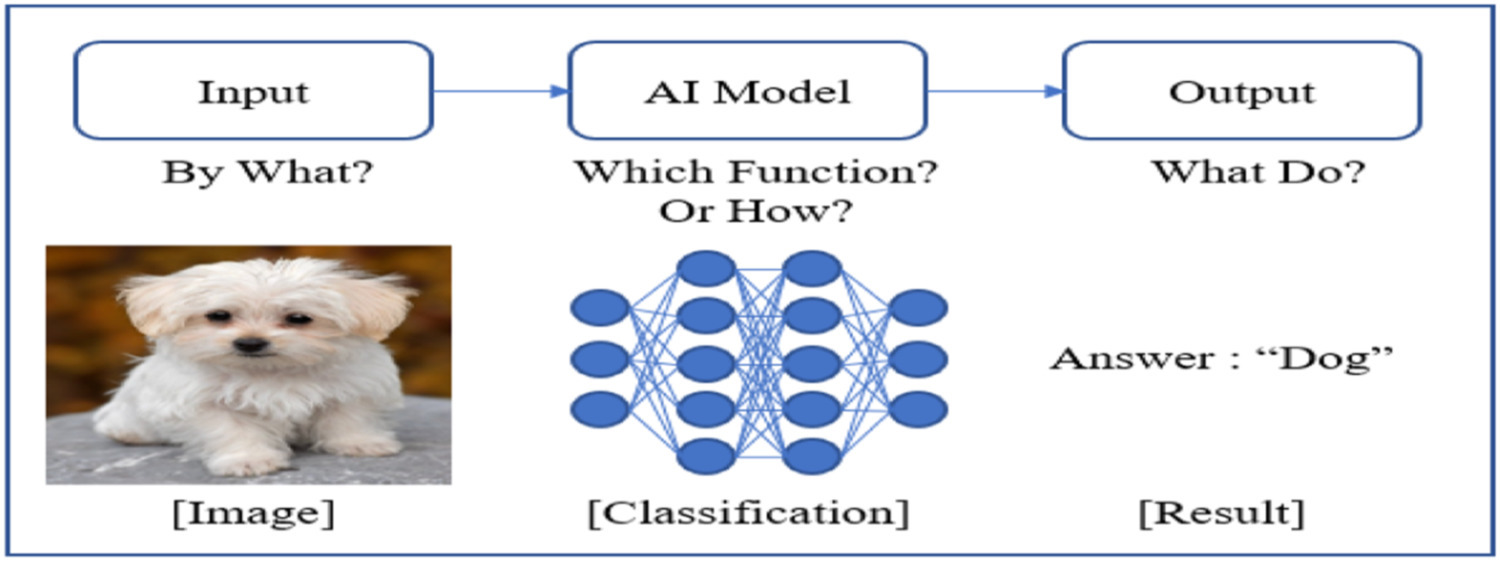
\includegraphics[width=0.5\textwidth]{image/fig 1.png}
                    \caption{مفهوم ساختار IMO}
                    \label{fig:fig_1}
            
                \end{figure}

            \subsubsection{چرا باید از ساختار IMO استفاده کرد؟}

                ساختار IMO یک ساختار منطقی است که ورودی و خروجی را به اطراف یک مدل هوش مصنوعی مرکز می‌کند. دلیل استفاده از ساختار IMO این است که یک مدل هوش مصنوعی نتیجه فناوری هوش مصنوعی است که از طریق داده و الگوریتم‌ها آموزش دیده شده است و موضوع عملکرد هوش مصنوعی است. حتی اگر چندین مدل هوش مصنوعی در سیستم راه‌اندازی و عمل کنند، هر مدل هوش مصنوعی از طریق ساختار IMO خود عمل می‌کند. ورودی مورد نیاز برای عملکرد مدل هوش مصنوعی همان معنی داده‌های مورد نیاز برای یادگیری یا عملکرد مدل هوش مصنوعی را دارد. خروجی نتیجه فناوری هوش مصنوعی است که مدل هوش مصنوعی از طریق داده‌های ورودی خروجی می‌دهد. به طور کلی، تمام ملاحظات طراحی برای پیاده‌سازی عملکرد هوش مصنوعی می‌تواند از طریق ساختار IMO مشتق شود. بنابراین، از منظر فنی، می‌توان ساختار IMO را به عنوان آغاز و پایان تشکیل فناوری هوش مصنوعی در نظر گرفت، و شناسایی ملاحظات طراحی برای فناوری هوش مصنوعی از طریق ساختار IMO منطقی به نظر می‌رسد.
    
            \subsubsection{ملاحظات فنی برای طراحی معماری سیستم هوش مصنوعی با استفاده از ساختار IMO}

                در این بخش، ملاحظات فنی برای طراحی سیستم‌ها و فناوری هوش مصنوعی با استفاده از ساختار IMO را شرح می دهیم. فناوری هوش مصنوعی به طور کلی به دو مرحله تقسیم می شود: فرآیند دستیابی به مدل های هوش مصنوعی و فرآیند بهره برداری از آنها. ساختار IMO در هر دو این مراحل گنجانده شده است، اما تفاوت در محیط است. محیطی که فرآیند دستیابی به مدل‌های هوش مصنوعی در آن انجام می‌شود، عمدتاً یک محیط آزمایشگاهی یا تحقیقاتی است، در حالی که محیطی که مدل هوش مصنوعی در آن اجرا می‌شود، سیستم واقعی است که مدل هوش مصنوعی در آن مستقر شده است. این تفاوت های محیطی در نهایت بر داده های مورد استفاده برای به دست آوردن مدل هوش مصنوعی و عملکرد مدل هوش مصنوعی به دست آمده تأثیر می گذارد. اگر این تفاوت‌ها در طول طراحی معماری نادیده گرفته شوند، مدل هوش مصنوعی ممکن است الزامات عملکرد را در مرحله اکتساب برآورده کند اما در مرحله عملیات واقعی سیستم نتواند آنها را برآورده کند. برای جلوگیری از این امر، در این مطالعه، ساختار IMO را از محیطی که سیستم هوش مصنوعی توسعه‌یافته در آن کار خواهد کرد، شناسایی کرده و از آن برای مشخص کردن الزامات فنی مرتبط با ساختار IMO در فرآیند دستیابی به مدل هوش مصنوعی استفاده می‌کنیم. برای نشان دادن اعتبار رویکردمان، توضیح می‌دهیم که چگونه ساختار IMO از نظر تئوری در هر دو فناوری هوش مصنوعی و دیدگاه‌های سیستم وجود دارد و آنچه باید بر اساس آن طراحی شود.

                \paragraph*{3.1.3.1}{دیدگاه فناوری هوش مصنوعی}
                
                    به دست آوردن فناوری هوش مصنوعی در نهایت به معنای به دست آوردن یک مدل هوش مصنوعی با عملکردهای مورد نظر است. فناوری‌های هوش مصنوعی به طور معمول به یادگیری نظارت شده، یادگیری بدون نظارت و یادگیری تقویتی تقسیم می‌شوند. فرآیند به دست آوردن این فناوری‌های هوش مصنوعی شامل به دست آوردن و عملکرد مدل‌های هوش مصنوعی است. شکل 2 هر فرآیند، روابط آن‌ها و مکان ساختار IMO را نشان می‌دهد. از آنجایی که فناوری هوش مصنوعی اساساً فناوری نرم‌افزاری است، زبان پایتون و دستورات کراس [20] برای توصیف آن استفاده شده است.

                    اولاً، همانطور که در سمت چپ شکل 2 نشان داده شده است، فرآیند به دست آوردن یک مدل هوش مصنوعی به طور کلی شامل سه مرحله است: آماده‌سازی آزمایش، طراحی الگوریتم هوش مصنوعی، آموزش و اعتبارسنجی، که معمولاً در یک محیط آزمایشگاهی انجام می‌شود. در مرحله آماده‌سازی آزمایش، داده‌های مورد نیاز برای یادگیری نظارت شده/بدون نظارت یا محیطی برای یادگیری تقویتی آماده می‌شود. سپس، در مرحله طراحی الگوریتم هوش مصنوعی، ساختار دقیق معماری IMO برای به دست آوردن مدل هوش مصنوعی طراحی می‌شود. ورودی‌ها به شکل شکل یا ابعادی که در الگوریتم هوش مصنوعی استفاده خواهد شد، طراحی می‌شوند. به عنوان مثال، در یادگیری نظارت شده/بدون نظارت، داده‌های پیش‌پردازش شده با اشکال یا ابعاد مشخص از تصاویر، صدا، یا متن به طور معمول استفاده می‌شود. این همچنین در مورد یادگیری تقویتی صادق است. با این حال، در یادگیری تقویتی، داده‌های به دست آمده از طریق وسایل مشاهده موجود در محیط طراحی شده برای عامل مانند دوربین‌ها یا رادارها استفاده می‌شود. الگوریتم‌های هوش مصنوعی از ترکیب لایه‌های شبکه عصبی مصنوعی مانند CNN، LSTM و Batchnormalization برای انجام عملکردهای مورد نظر تشکیل شده‌اند. سمت چپ شکل 2 مثالی از کد منبع کلی را نشان می‌دهد که الگوریتم یادگیری نظارت شده را به آن کمک می‌کند تا درک شود. خروجی عملکرد مورد نیاز توسط مدل هوش مصنوعی را نشان می‌دهد. به عنوان مثال، در یادگیری نظارت شده، این ممکن است یک برچسب مانند "سگ" باشد، و در یادگیری تقویتی، این ممکن است یک عمل مانند "حرکت به بالا" یا "حرکت به پایین" باشد. در نهایت، در مرحله آموزش و اعتبارسنجی، وظایف آموزش و اعتبارسنجی تکراری با استفاده از داده‌های (یا محیط) آماده‌شده و الگوریتم هوش مصنوعی انجام می‌شود. در یادگیری نظارت شده، یادگیری هوش مصنوعی عمدتاً با کاهش تفاوت بین خروجی الگوریتم هوش مصنوعی و حقیقت انجام می‌شود. در یادگیری بدون نظارت، یادگیری هوش مصنوعی بدون برچسب انجام می‌شود، اما هوش مصنوعی توزیع یا ویژگی‌های داده‌ها را به درستی یاد می‌گیرد تا به عنوان هدف توسط معمار هوش مصنوعی مورد نظر دسته‌بندی شود. در یادگیری تقویتی، یادگیری هوش مصنوعی با بیشینه کردن پاداش تجمعی حاصل از خروجی الگوریتم هوش مصنوعی در محیط انجام می‌شود. این مرحله تا زمانی که مدل هوش مصنوعی به معیارهای عملکرد کافی مانند دقت برسد، تکرار می‌شود. در نهایت، محصول نهایی کلیه فرآیند به دست آوردن یک مدل هوش مصنوعی، یک مدل هوش مصنوعی آموزش‌دیده به خوبی است.

                    دوماً، همانطور که در سمت راست شکل 2 نشان داده شده است، فرآیند عملکرد مدل هوش مصنوعی شامل دو مرحله است: بارگذاری مدل هوش مصنوعی و عملکرد مدل هوش مصنوعی. این فرآیند در یک سیستم در یک محیط عملیاتی واقعی انجام می‌شود. در مرحله بارگذاری مدل هوش مصنوعی، وظیفه بارگذاری مدل هوش مصنوعی آموزش‌دیده و الگوریتم‌های آن به حافظه سیستم است. سپس، در مرحله عملکرد مدل هوش مصنوعی، سیستم با استفاده از مقادیر ورودی از سیستم و مدل هوش مصنوعی بارگذاری شده، مقادیر خروجی را پیش‌بینی می‌کند. بزرگترین تفاوت بین این مرحله و مرحله به دست آوردن مدل هوش مصنوعی، داده است. در حالی که در فرآیند به دست آوردن مدل هوش مصنوعی از داده‌های آماده استفاده می‌شود، فرآیند عملکرد مدل هوش مصنوعی داده‌های ورودی را از سیستم واقعی دریافت می‌کند.

                    \begin{figure}[htbp]

                        \centering
                        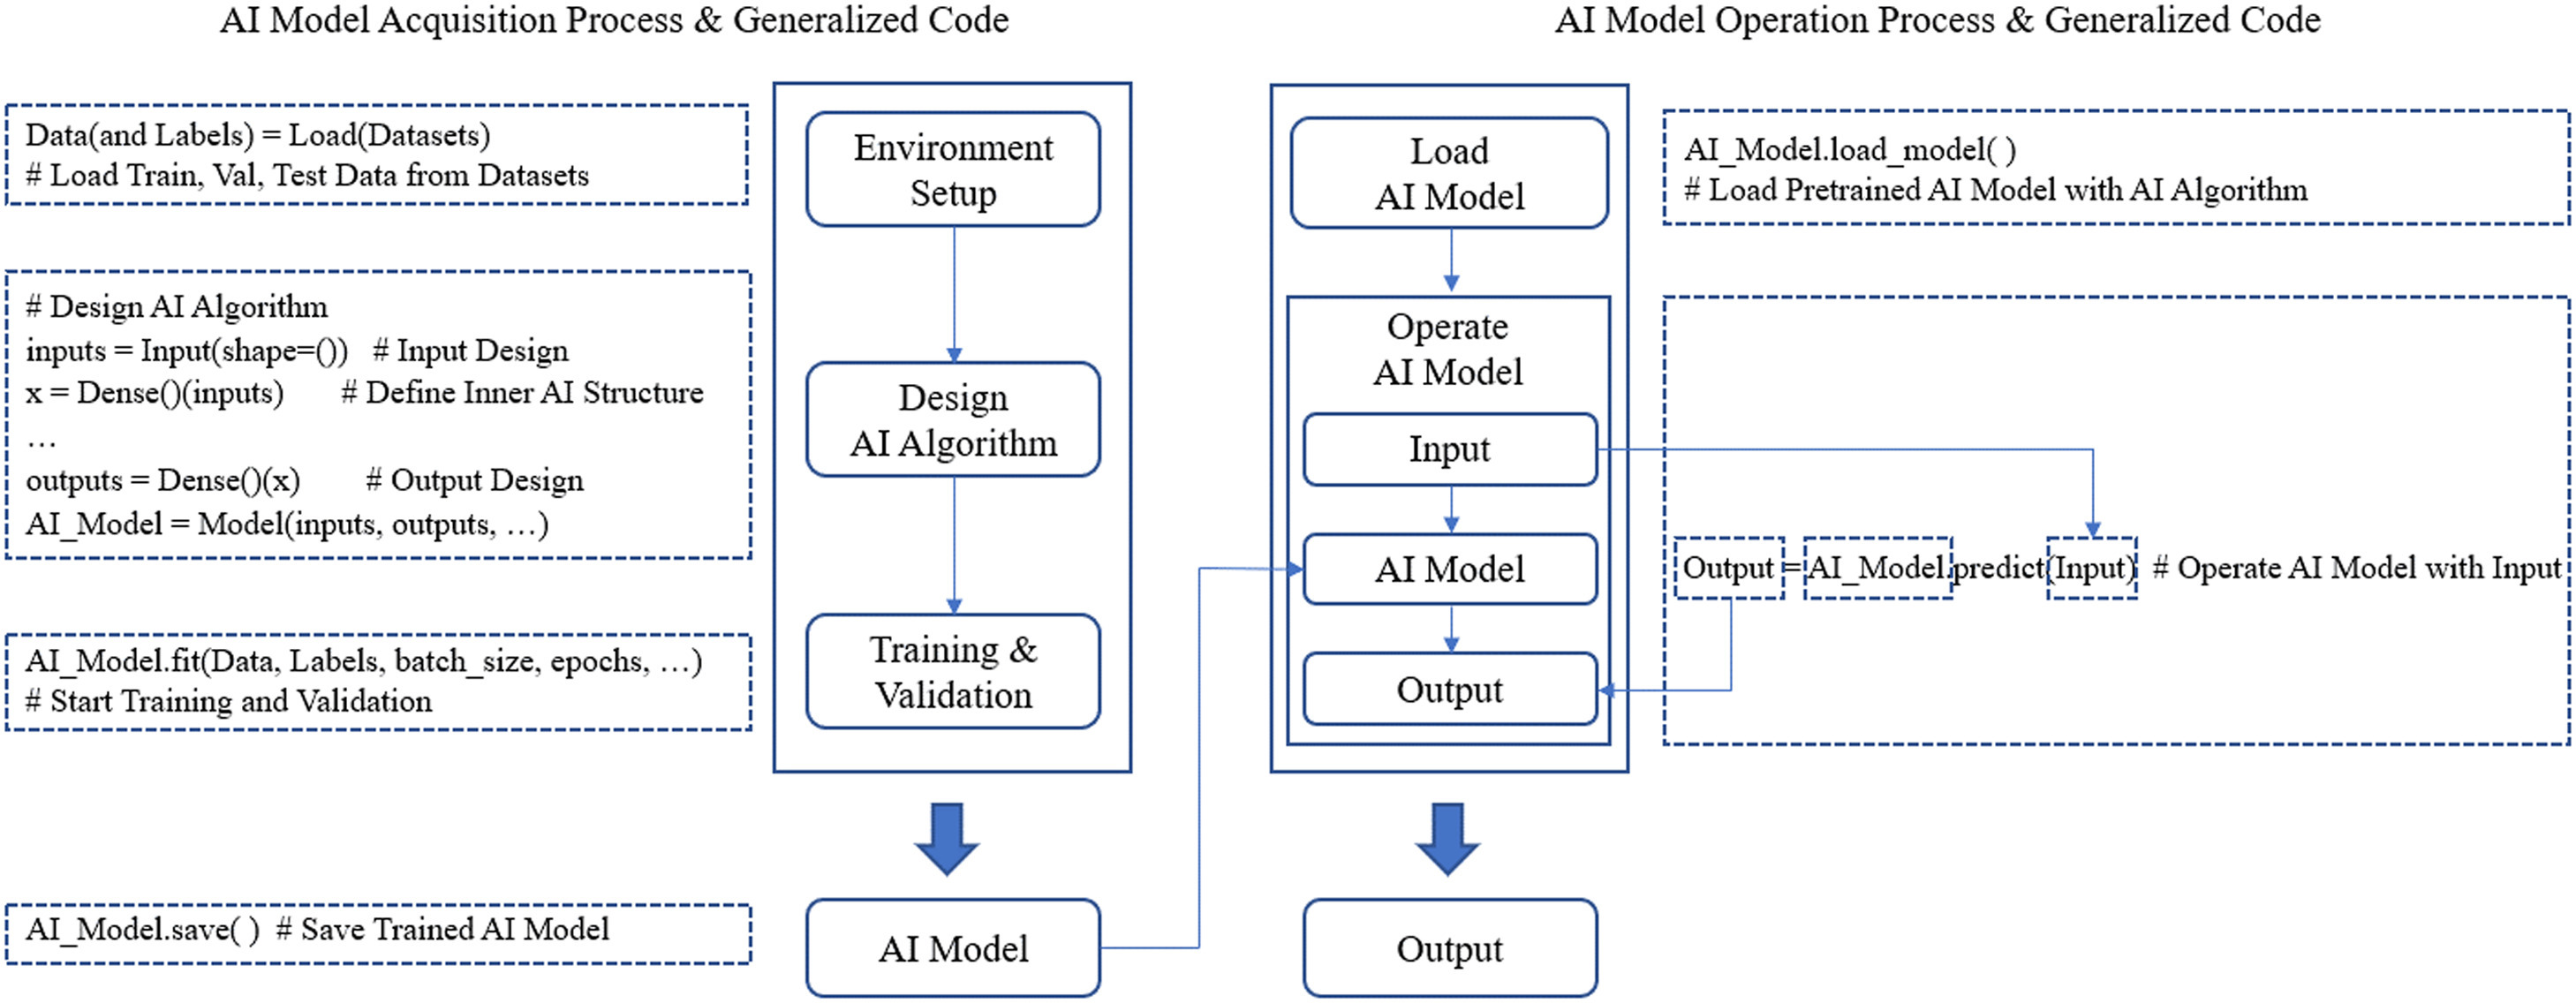
\includegraphics[width=0.8\textwidth]{image/fig 2.png}
                        \caption{فرآیند کسب و عملیات یک مدل هوش مصنوعی و موقعیت ساختار IMO}
                        \label{fig:fig_2}
                    
                    \end{figure}

                \paragraph*{3.1.3.2}{دیدگاه سیستمی}

                    سیستم دارای یک معنای گسترده است [[5], [6], [7],21,22]، اما به طور کلی می‌توان آن را به عنوان یک مجموعه متنوع از عناصر مرتبط که با همکاری با یکدیگر برای دستیابی به یک هدف مشترک کار می‌کنند، تعریف کرد. بسته به قصد طراح، سیستم از ترکیبی از عناصری که در سطوح مختلف موجود هستند، مانند زیرسیستم‌ها، اجزا و بخش‌ها، از طریق فرآیند تجزیه و تحلیل سیستم تشکیل شده است. در این زمینه، ممکن است اجزا به اشکال مختلفی مانند برقی، کنترل‌کننده‌ها، نرم‌افزار (SW) یا اشکال دیگر تعریف شوند، بسته به نقش اختصاص یافته در طراحی سیستم به عنوان یک زیرسیستم یا عنصر سطح پایین‌تر سیستم. برای کاهش پیچیدگی، توصیف زیرعناصر زیر سطح قسمت‌ها در این مطالعه حذف شده است. همانطور که قبلاً گفته شد، فناوری هوش مصنوعی یک فناوری نرم‌افزاری است که برای انجام عملکردهای خاصی مانند شناخت، تولید و رفتار طراحی شده است، و خروجی آن یک مدل هوش مصنوعی است. بنابراین، فناوری هوش مصنوعی در ماژول SW که مدل هوش مصنوعی استفاده می‌شود و در سطح اجزا SW نماینده می‌شود، وجود دارد. در این مقاله، آن را به عنوان یک مؤلفه هوش مصنوعی نام می‌دهیم. به طور خلاصه، از دیدگاه سیستم، یک سیستم هوش مصنوعی می‌تواند به عنوان یک سیستم با یک یا چند مؤلفه هوش مصنوعی تعریف شود، و یک مؤلفه هوش مصنوعی یک مؤلفه سیستم با یک یا چند ساختار IMO است. شکل 3 سلسله مراتب کلی سیستم هوش مصنوعی و چگونگی وجود ساختار IMO را نشان می‌دهد. ساختار SW شامل مدل هوش مصنوعی در شکل 3 یک مؤلفه هوش مصنوعی است، و سیستم و زیرسیستم حاوی مؤلفه هوش مصنوعی به ترتیب به عنوان سیستم‌های هوش مصنوعی و زیرسیستم‌های هوش مصنوعی نمایش داده می‌شوند.

                    \begin{figure}[htbp]

                        \centering
                        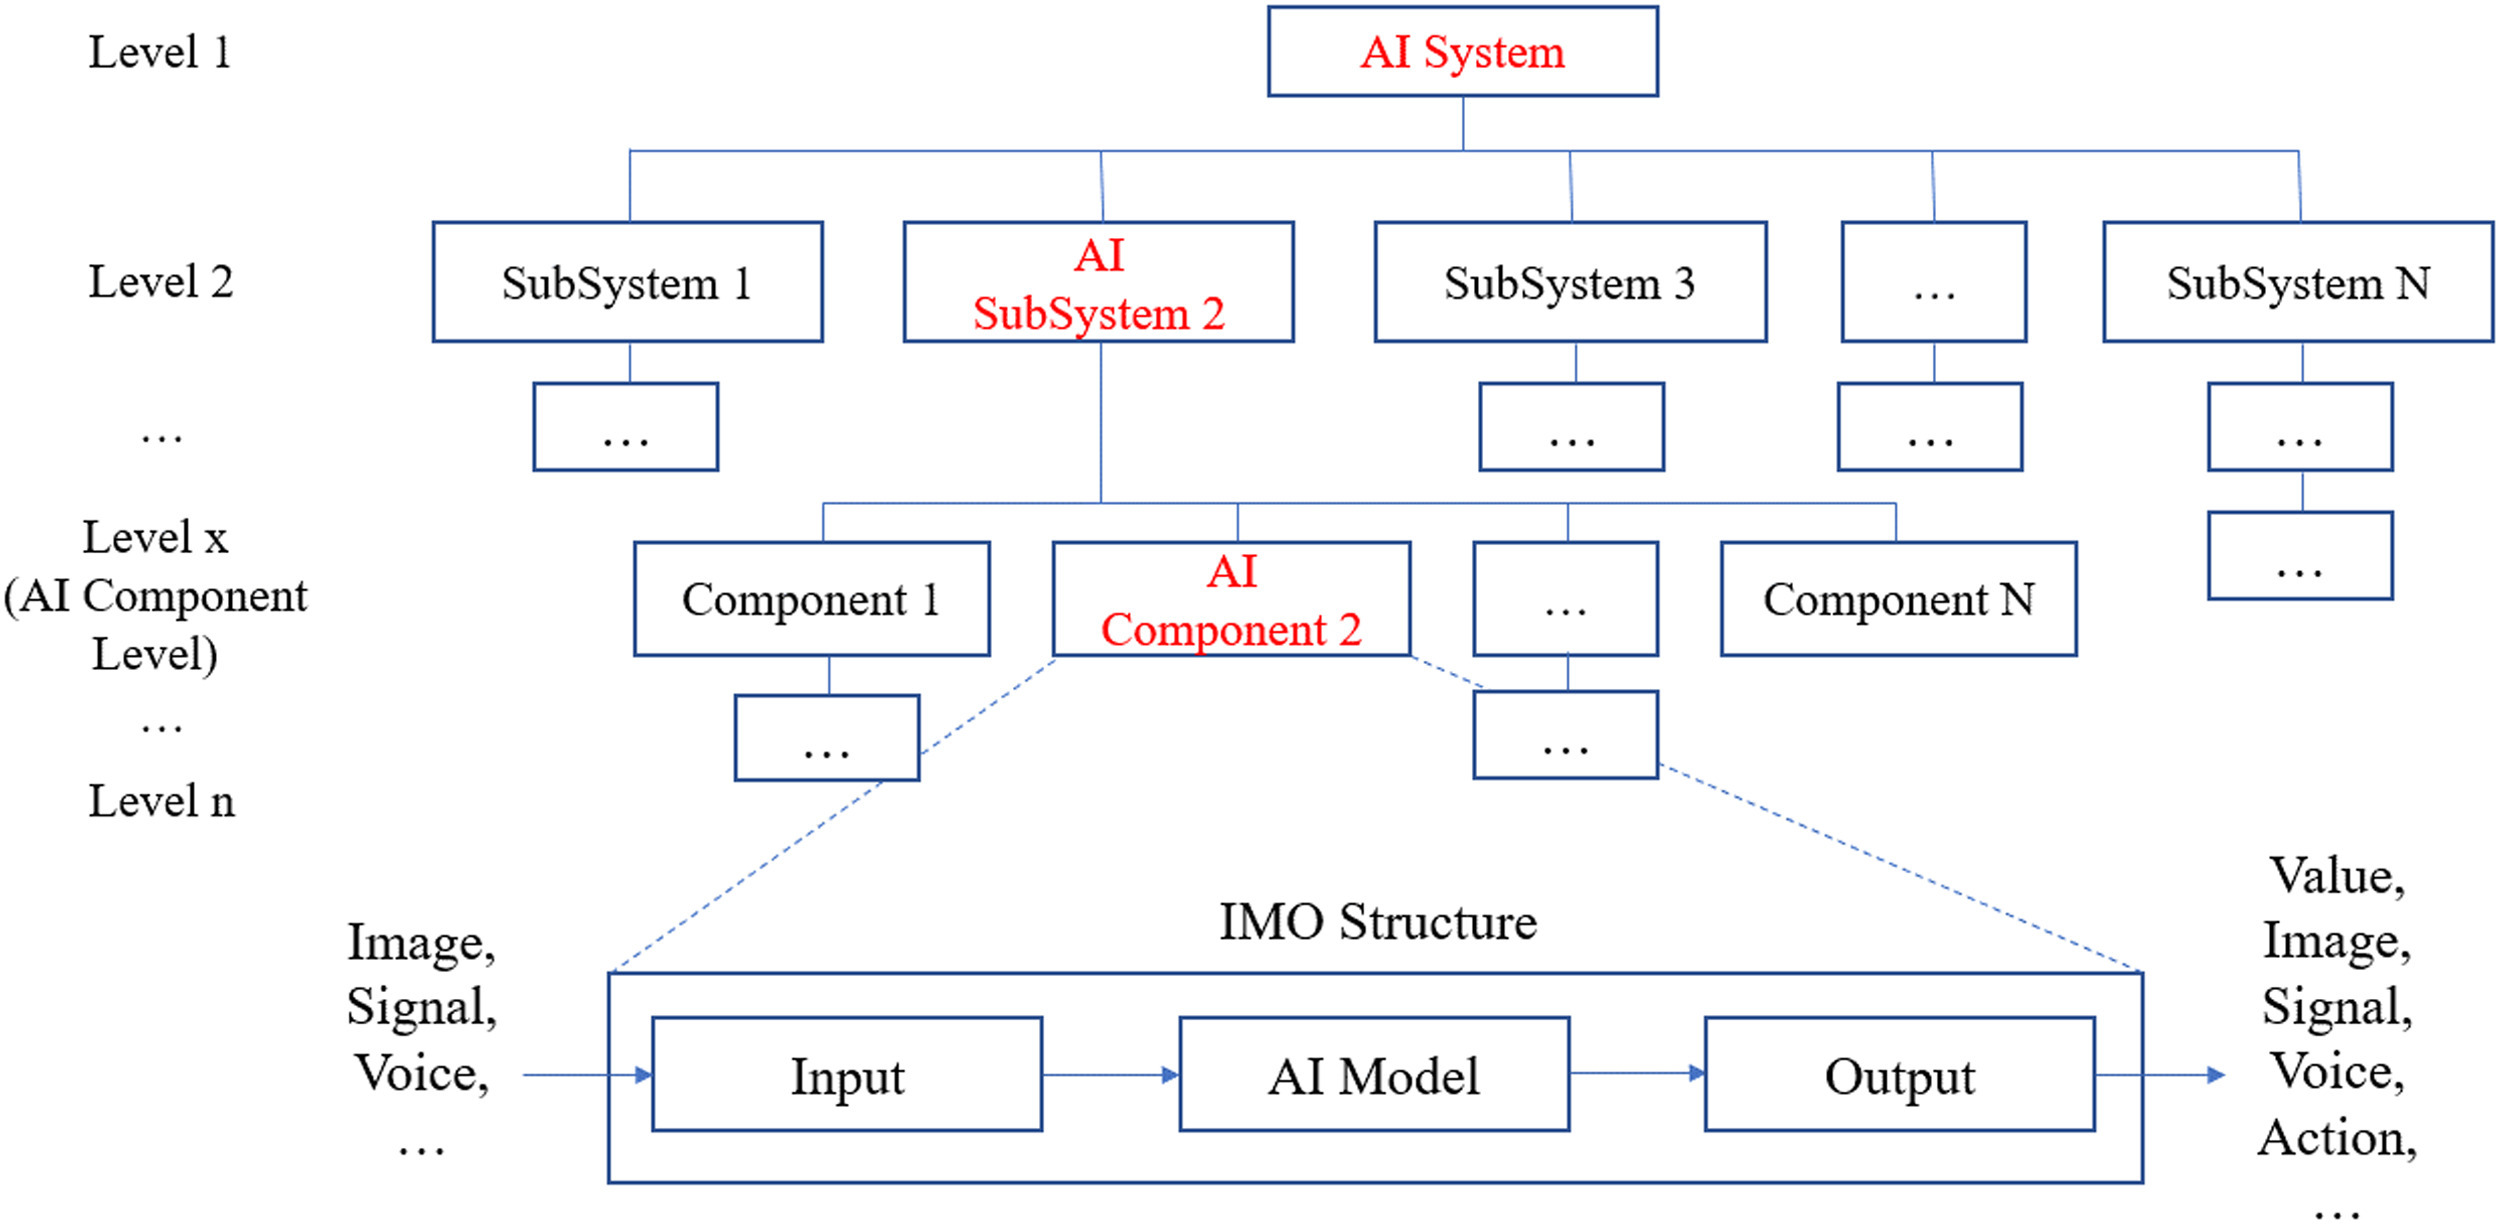
\includegraphics[width=0.6\textwidth]{image/fig 3.png}
                        \caption{سلسله مراتب یک سیستم هوش مصنوعی تعمیم یافته و مکان ساختار IMO}
                        \label{fig:fig_3}
                    
                    \end{figure}

                \paragraph*{3.1.3.3}{ملاحظات فنی برای طراحی معماری سیستم هوش مصنوعی}

                    در این بخش، ما در مورد ملاحظات فنی که باید هنگام ساختاردهی یک معماری سیستم هوش مصنوعی از طریق ساختار IMO شناسایی یا طراحی شوند توضیح می‌دهیم. ملاحظات فنی پیشنهاد شده در این مطالعه شامل چهار مورد می‌شود: داده یا محیط، الگوریتم هوش مصنوعی و خروجی، عملکرد هوش مصنوعی و الزامات مؤلفه هوش مصنوعی.

                    \begin{itemize}
                        
                        \item داده یا محیط: داده و محیط پیش‌نیازهای ضروری برای یادگیری الگوریتم‌های هوش مصنوعی هستند و با قسمت I از ساختار IMO ارتباط دارند. به طور کلی، فناوری هوش مصنوعی برای یادگیری نیاز به حجم زیادی از داده دارد و آماده‌سازی داده بیشترین زمان را در توسعه مدل هوش مصنوعی به خود اختصاص می‌دهد. علاوه بر این، داده تأثیر مستقیمی بر عملکرد مدل‌های هوش مصنوعی دارد. بنابراین، طراحی الزامات روشن برای داده یا محیط هنگام طراحی عملکرد هوش مصنوعی سیستم بسیار حیاتی است. همانطور که در بخش 3.1.3.1 مشاهده می‌شود، تفاوت اصلی بین فرآیندهای به دست آوردن و عملیات مدل‌های هوش مصنوعی داده ورودی است. در فرآیند به دست آوردن یک مدل هوش مصنوعی، ورودی داده آماده یا اطلاعاتی است که در یک محیط آماده‌سازی شده به دست آمده و عملکرد مدل هوش مصنوعی آموزش دیده را تعیین می‌کند. با این حال، در زمان عملیات مدل هوش مصنوعی، ورودی داده یا اطلاعاتی است که در محیط عملیاتی واقعی سیستم به دست آمده و عملکرد واقعی سیستم هوش مصنوعی را تعیین می‌کند. اگر داده یا اطلاعاتی که از محیط عملیاتی واقعی به دست می‌آید با داده یا محیطی که برای به دست آوردن مدل هوش مصنوعی استفاده شده است متفاوت باشد، مدل هوش مصنوعی آموزش دیده شده ممکن است عملکرد ضعیف یا رفتارهای نامطلوبی داشته باشد. بنابراین، هنگام طراحی معماری سیستم هوش مصنوعی، داده یا محیط باید بر اساس تجزیه و تحلیل محیط عملیاتی سیستم واقعی مشتق و تأیید شود.

                        \item الگوریتم‌های هوش مصنوعی و خروجی: به عنوان مواردی که می‌توانند به طور مستقیم به الزامات ذینفعان برای عملکرد هوش مصنوعی نقش ببینند، با مؤلفه‌های M و O از ساختار IMO مرتبط هستند. الگوریتم‌های هوش مصنوعی به الزامات ذینفعان برای "کدام عملکرد" سیستم هوش مصنوعی باید انجام دهد نقش می‌بیند، که ممکن است شامل عملکردهایی مانند طبقه‌بندی، شناسایی و تولید باشد. خروجی به الزامات ذینفعان برای "چگونگی ارائه عملکرد" نقش می‌بیند. به عنوان مثال، اگر الزامات ذینفعان برای شناسایی آبجکت‌ها به صورت زمان واقعی از تصاویر باشد، عملکرد هوش مصنوعی "شناسایی" خواهد بود و خروجی "موقعیت آبجکت در تصویر" خواهد بود. این‌ها می‌توانند به صورت محکم به برخی الگوریتم‌های هوش مصنوعی خاص مانند YOLO یا Faster R-CNN، که می‌توانند عملکرد "شناسایی" را انجام دهند، از طریق فرآیند طراحی معماری دقیق مواد شوند. و خروجی می‌تواند به اشکال مختلفی مانند "برچسب" و "جعبه‌ی محدود" نمایش داده شود.

                        \item کارایی هوش مصنوعی: به عملکرد یک مدل آموزش دیده هوش مصنوعی اشاره دارد و با عناصر M و O از ساختار IMO ارتباط دارد. روش‌های مختلفی برای اندازه‌گیری عملکرد یک مدل هوش مصنوعی وجود دارد که به نوع و هدف الگوریتم هوش مصنوعی بستگی دارد. بنابراین، الزامات عملکرد هوش مصنوعی باید روش اندازه‌گیری عملکرد مناسبی را انتخاب کنند که در حد امکان نیازهای ذینفعان را برآورده کند. به عنوان مثال، mAP به طور اصلی برای شناسایی آبجکت [23] استفاده می‌شود و WER به طور اصلی برای تشخیص گفتار استفاده می‌شود. با این حال، در یادگیری تقویتی، عملکرد یک عامل می‌تواند بسته به محیط پویایی تغییر کند، و در حال حاضر هیچ راه روشنی برای مقایسه عملکرد عوامل آموزش دیده وجود ندارد. تلاش‌های مختلفی برای حل این مسئله وجود دارد. اولین راه حل ایجاد بسیاری از محیط‌های استاندارد است که مشکلات هر دامنه را به وضوح نشان دهند. دومین راه حل توسعه انواع مختلفی از سناریوهای آزمایش استاندارد برای عوامل یادگیری تقویتی در هر محیط استاندارد است. در نهایت، نمودار پاداش تجمعی یک مدل هوش مصنوعی که در محیط‌ها و سناریوهای آزمایش استاندارد اندازه‌گیری شده‌است، می‌تواند به عنوان یک شاخص عملکرد پایداری مورد استفاده قرار گیرد. این نمودار پاداش هر مقدار پاداشی را که عامل در طول فرآیند یادگیری به دست آورده است نمایش می‌دهد. اگر این نمودار ارزش‌های پاداش بالایی را در محیط‌ها و سناریوهای آزمایش استاندارد مختلف به طور پایدار حفظ کند، مدل هوش مصنوعی آموزش دیده شده را پایدار می‌توان در نظر گرفت.

                        \item الزامات مؤلفه‌های هوش مصنوعی: به الزامات سطح سیستم برای عملکرد مدل‌های هوش مصنوعی تهیه شده می‌پردازد، که شامل مؤلفه‌های نرم‌افزاری (SW) مانند سیستم عامل (OS) و مؤلفه‌های سخت‌افزاری (HW) مانند واحد پردازش مرکزی (CPU) و حافظه دسترسی تصادفی (RAM) می‌شود. الزامات مؤلفه‌های هوش مصنوعی با طراحی منابع محاسباتی لازم مرتبط بوده و در نهایت بر روی هزینه تولید سیستم‌های هوش مصنوعی تأثیر می‌گذارد. به طور کلی، برای فرآیند تهیه مدل هوش مصنوعی، منابع محاسباتی با عملکرد بالا لازم است. با این حال، برای فرآیند عملکرد مدل هوش مصنوعی، منابع محاسباتی با عملکرد نسبتاً پایین لازم است. در فرآیند تهیه مدل هوش مصنوعی، داده‌ها یا محیطی که برای آموزش آماده شده‌اند، به حافظه سیستم بارگذاری شده و وزن‌های مدل هوش مصنوعی به‌طور مکرر محاسبه و به‌روزرسانی می‌شود. در حالی که فرآیند عملکرد مدل هوش مصنوعی تنها نیاز به استنتاج با استفاده از مدل هوش مصنوعی آموزش دیده دارد. بسیاری از مطالعات در حال انجام است برای پوشش دادن نقص منابع محاسباتی با عملکرد بالا برای عملکرد مدل‌های هوش مصنوعی. به عنوان مثال، مطالعات مختلفی عملکرد استنتاج به‌روز مدل هوش مصنوعی حتی در محیط‌های با عملکرد پایین مانند CPUs یا گوشی‌های همراه را نشان داده‌اند. بنابراین، هنگام طراحی معماری سیستم، مشخصات HW مناسب برای عملکرد مدل هوش مصنوعی آموزش دیده باید مدنظر قرار گیرد تا هزینه را در نظر بگیرد، یا تکنولوژی‌های هوش مصنوعی که حتی در محیط‌های با عملکرد پایین هم قابل عملیات هستند، باید مورد بررسی قرار گیرد.

                    \end{itemize}
        
        \subsection{فرآیند طراحی معماری سیستم هوش مصنوعی پیشنهادی}

            در این بخش، فرآیند طراحی معماری سیستم هوش مصنوعی را با تمرکز بر روی ساختار IMO شرح می‌دهیم. روش طراحی معماری پیشنهادی هدفش شناسایی و طراحی الزامات فنی برای سیستم‌ها و فناوری‌های هوش مصنوعی لازم از فعالیت‌های عملیاتی آینده است که می‌توانند به دستاوردهای سازمان برسند.

            \subsubsection{فرآیند اساسی}

                منهجی که ما ارائه داده‌ایم از سه فعالیت تشکیل شده است: تعریف مسئله، راه‌حل هوش مصنوعی سیستمی، و راه‌حل فنی هوش مصنوعی. شکل ۴ فرآیند پیشنهادی طراحی معماری سیستم هوش مصنوعی را نشان می‌دهد. فعالیت اول تعریف مسئله است. هدف این فعالیت مشخص کردن وضعیت مسئله و جایگزینی است که سازمان می‌خواهد از منظر عملیاتی به آن پرداخته شود. در این مرحله، مسائل سازمان و نقش‌های هوش مصنوعی برای حل مسائل شناسایی می‌شوند. فعالیت دوم، راه‌حل هوش مصنوعی سیستمی، هدف طرح‌های مشخص‌شده که می‌توانند الزامات سازمان را که از منظر عملیاتی شناسایی شده‌اند، از دیدگاه سیستمی به تجسم در آورد. در این مرحله، ساختار سیستم و الزامات عنصر هوش مصنوعی که می‌توانند نقش‌های هوش مصنوعی شناسایی شده را انجام دهند، مشخص می‌شود. فعالیت آخر، راه‌حل فنی هوش مصنوعی، هدف تشخیص الزامات فنی برای به دست آوردن فناوری هوش مصنوعی است که می‌تواند نقش‌های هوش مصنوعی شناسایی شده را انجام دهد. در این مرحله، داده‌ها و عملکردهای هوش مصنوعی مورد نیاز برای توسعه مدل‌های هوش مصنوعی که در سیستم واقعی منافع استفاده خواهند شد، مشخص می‌شود.

                \begin{figure}[htbp]

                    \centering
                    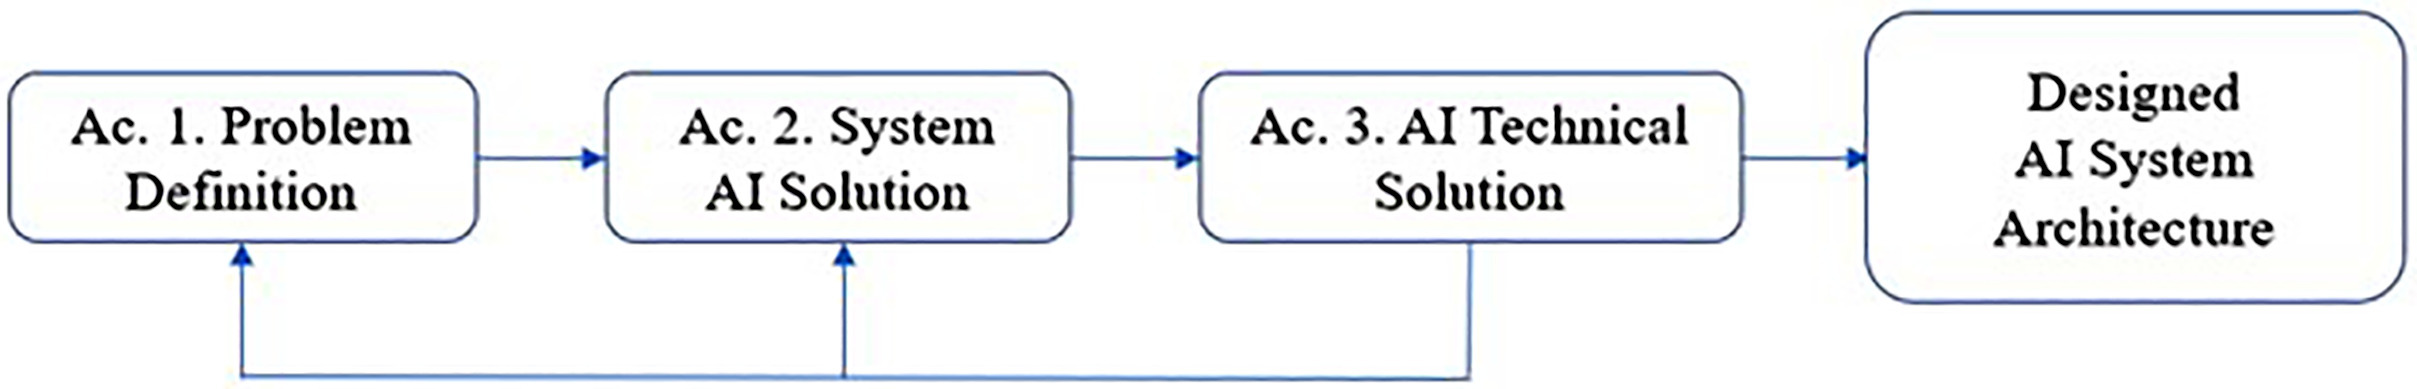
\includegraphics[width=0.6\textwidth]{image/fig 4.png}
                    \caption{فرآیند اساسی روش طراحی معماری سیستم هوش مصنوعی پیشنهادی}
                    \label{fig:fig_4}
                
                \end{figure}
            
                همانطور که در فصل 2 بررسی شد، طراحی معماری از طریق فعالیت‌های مهندسی سیستم معمولاً بر روی راه‌حل‌های سیستم تمرکز دارد. به عنوان مثال، چارچوب‌های موجود مانند DoDAF روش‌هایی برای تعریف دیدگاه‌های مختلف عملیاتی یا سیستمی ارائه می‌دهند، اما دیدگاه‌های برای بیان فناوری‌ها مانند StdV خاص نیستند و روش‌های شرح روشنی فراهم نمی‌کنند. به عنوان نتیجه، مطالعات موجود با استفاده از چارچوب‌های معمولی در شناسایی فناوری‌های هوش مصنوعی انتزاع بالایی را نشان می‌دهند. برای رفع این محدودیت‌ها، منهج ما با استفاده از درنظر گرفتن الزامات فنی مشتق شده از ساختار IMO، فناوری‌های هوش مصنوعی را مشخص می‌کند. سه فعالیت تا زمان کامل شدن طراحی معماری مکرر می‌شوند، که منجر به طراحی نهایی معماری سیستم هوش مصنوعی می‌شود.

            \subsubsection{فرآیند دقیق}

                در این بخش، جزئیات فرآیند پیشنهادی منهج را توضیح می‌دهیم. شکل 5 رابطه میان سه فعالیت طراحی پیشنهادی را نشان می‌دهد. هر فعالیت طراحی از خروجی اصلی خود استفاده می‌کند. فرآیند طراحی پیشنهادی به صورت مکرر از طریق همکاری کارشناسان حوزه، سیستم و هوش مصنوعی انجام می‌شود تا خروجی‌های اصلی هر مرحله به اندازه کافی بهبود یابند.

                \begin{figure}[htbp]

                    \centering
                    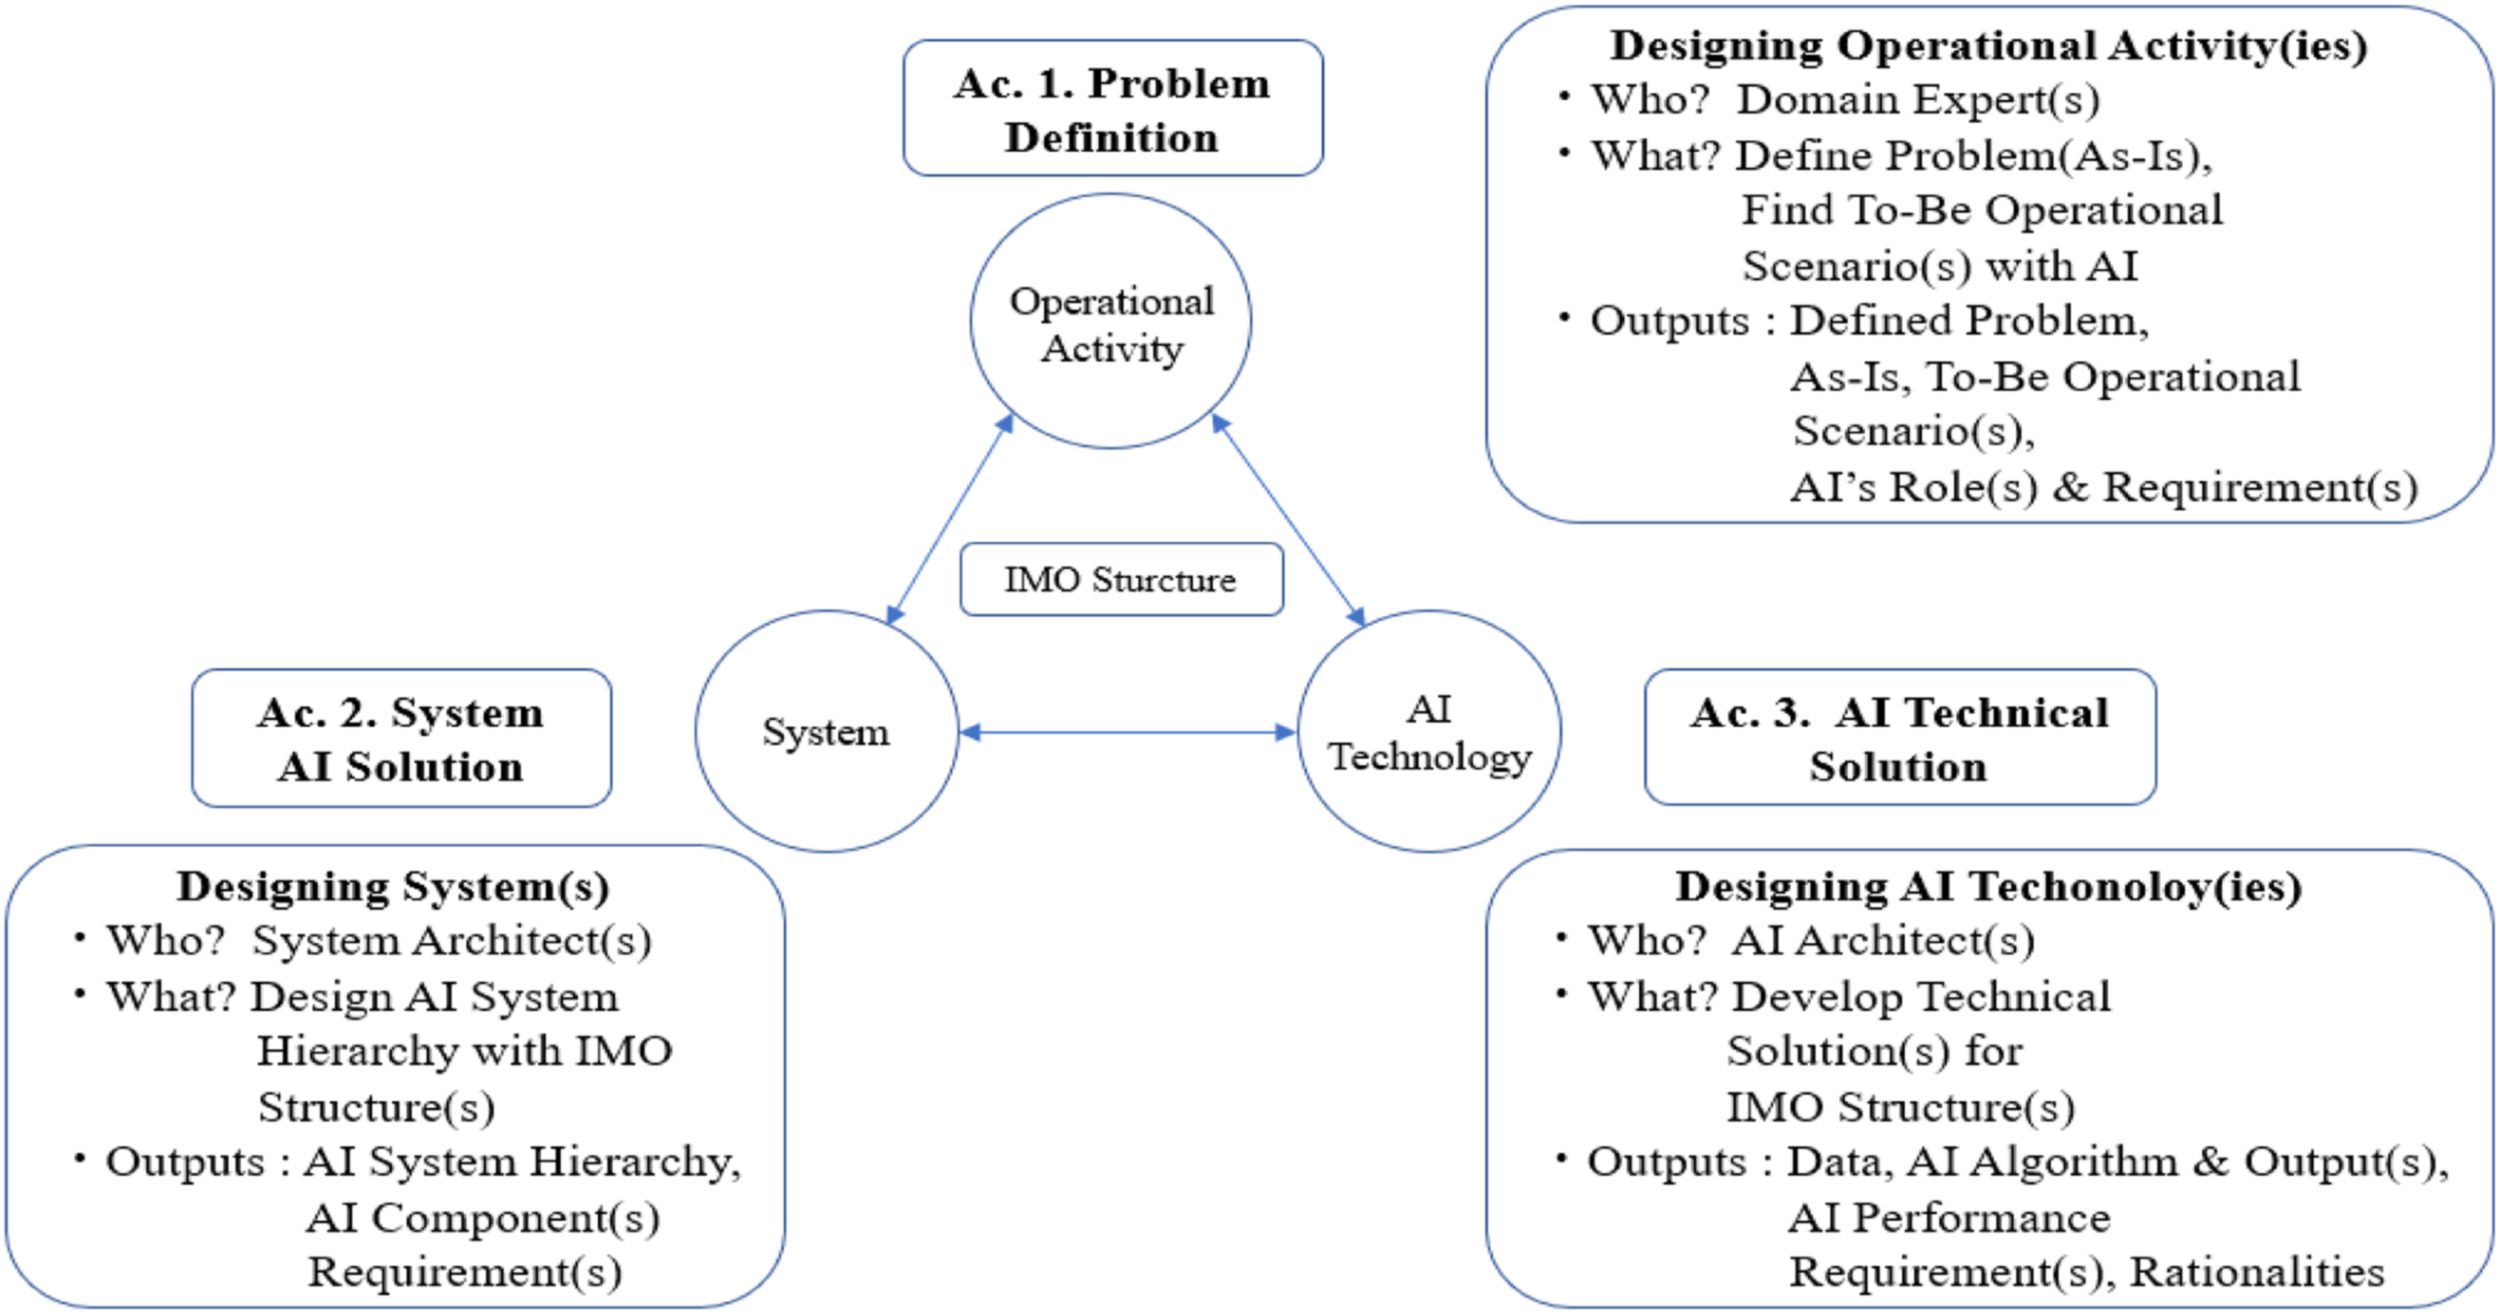
\includegraphics[width=0.8\textwidth]{image/fig 5.png}
                    \caption{رابطه متقابل بین سه فعالیت طراحی پیشنهادی}
                    \label{fig:fig_5}
                
                \end{figure}

                \paragraph{3.2.2.1}{مرحله تعریف مسئله Ac.1}

                    در مرحله تعریف مسئله، مسائلی که در حوزه تخصصی سازمان باید مورد توجه قرار گیرند، از طریق فعالیت‌های عملیاتی تعریف می‌شوند و نقش هوش مصنوعی بر اساس آن‌ها مشخص می‌شود. از آنجا که این مرحله به مسائل در حوزه تخصصی می‌پردازد، اصولاً توسط کارشناسان حوزه انجام می‌شود و از طریق چهار فعالیت جزئی انجام می‌شود که در شکل 6 زیر نشان داده شده است.

                    \begin{figure}[htbp]

                        \centering
                        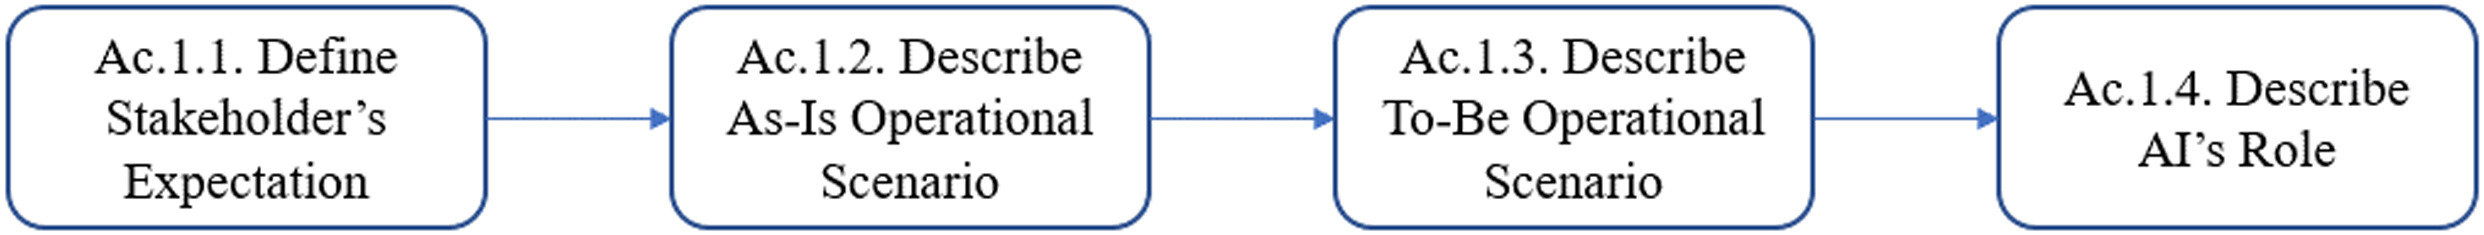
\includegraphics[width=0.8\textwidth]{image/fig 6.png}
                        \caption{رابطه متقابل بین سه فعالیت طراحی پیشنهادی}
                        \label{fig:fig_6}
                    
                    \end{figure}

                    جدول ۱ زیر نشان دهنده خروجی‌های اصلی است که باید در مرحله تعریف مسئله شناسایی شوند. شرح توضیحات جزئی هر فعالیت که خروجی‌های اصلی را مشخص می‌کند، به شرح زیر است.

                    \begin{table}[htbp]
                        
                        \centering
                        \caption{خروجی‌های اصلی مرحله تعریف مسئله}
                        \begin{tabularx}{\textwidth}{X}
                        
                            \specialrule{1pt}{1pt}{5pt}
                            \multicolumn{1}{c}{انتظارات ذینفعان [Ac.1.1.]} \\
                            \specialrule{0.5pt}{1pt}{1pt}
                            
                            شرح: مسئله‌هایی که باید با استفاده از هوش مصنوعی حل شوند را توصیف کنید یا تعریف کنید. \\
                            
                            \specialrule{0.5pt}{1pt}{5pt}
                            \multicolumn{1}{c}{سناریو(های) as-is [Ac.2.1.]} \\
                            \specialrule{0.5pt}{1pt}{1pt}
                            
                            شرح: مسائل فعلی که باید با استفاده از هوش مصنوعی حل شوند را به عنوان یک یا چند سناریو عملی از طریق روش‌های مناسب مانند EFFBD(s) و متن‌ها بیان کنید. \\
                            شرایط: عواملی که بر سناریو(های) عملی تأثیر می‌گذارند مانند زمان، فضا و سایر موارد را شرح دهید. \\
                            
                            \specialrule{0.5pt}{1pt}{5pt}
                            \multicolumn{1}{c}{سناریو(های) to-be [Ac.3.1.]} \\
                            \specialrule{0.5pt}{1pt}{1pt}
                            
                            شرح: بیان کنید سناریو(های) عملی آینده که مسئله(ها) با استفاده از هوش مصنوعی حل می‌شود(ند)، از طریق روش‌های مناسب مانند EFFBD(s) و متن. \\
                            شرایط: عواملی که بر سناریو(های) عملی تأثیر می‌گذارند، مانند زمان، فضا و سایر موارد را شرح دهید. \\
                            
                            \specialrule{0.5pt}{1pt}{5pt}
                            \multicolumn{1}{c}{نقش(های) هوش مصنوعی} \\
                            \specialrule{0.5pt}{1pt}{1pt}
                            
                            شرح: نقش(های) و اجرا کننده(ها) های هوش مصنوعی مورد نیاز برای سناریو(های) عملی آینده را (با در نظر گرفتن عنصر M و عنصر O از ساختار IMO) بیان کنید. \\
                            
                            \specialrule{1pt}{1pt}{1pt}
                            
                        \end{tabularx}
                    \end{table}



\end{document}